%#!pdflatex
\documentclass{standalone}
\usepackage[svgnames]{xcolor}
\usepackage{tikz}
\usetikzlibrary{arrows.meta, calc, backgrounds}
\begin{document}
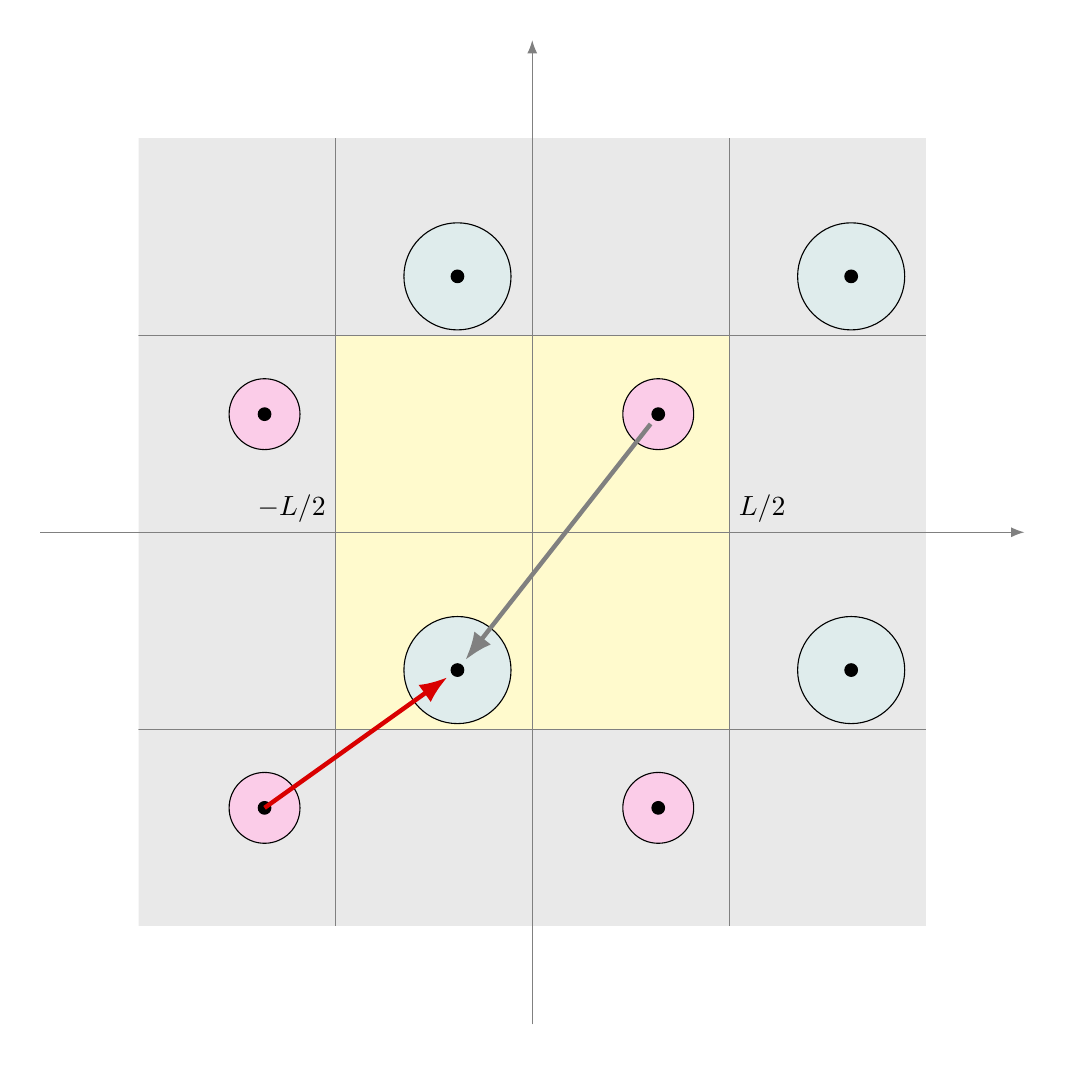
\begin{tikzpicture}[background rectangle/.style={fill=white}, show background rectangle]
\pgfmathsetmacro{\Lbox}{5}

\begin{scope}
\clip (-\Lbox, -\Lbox) rectangle ++(2*\Lbox, 2*\Lbox);

\foreach \x in {-1,0,1}
\foreach \y in {-1,0,1}
\fill [LightGray!50] (-0.5*\Lbox + \x*\Lbox, -0.5*\Lbox + \y*\Lbox) rectangle ++(\Lbox, \Lbox);

\fill [LemonChiffon] (-0.5*\Lbox, -0.5*\Lbox) rectangle ++(\Lbox, \Lbox);

\foreach \x in {-1,1,0}
{
\foreach \y in {-1,1,0}
{
\draw [gray] (-0.5*\Lbox + \x*\Lbox, -0.5*\Lbox + \y*\Lbox) rectangle ++(\Lbox, \Lbox);

\filldraw [draw=black, fill=magenta!20]   ( 0.32*\Lbox + \x*\Lbox,  0.30*\Lbox + \y*\Lbox) node (Pred) {}  circle [radius=0.45];
\filldraw [draw=black, fill=CadetBlue!20] (-0.19*\Lbox + \x*\Lbox, -0.35*\Lbox + \y*\Lbox) node (Pblue) {} circle [radius=0.68];

\filldraw [draw=black, fill=black] (Pred)  circle [radius=0.08];
\filldraw [draw=black, fill=black] (Pblue) circle [radius=0.08];
}
}
\end{scope}
\draw [-Latex, ultra thick, gray]          (Pred) -- (Pblue);
\draw [-Latex, ultra thick, red!85!black]  ($(Pred) - (\Lbox, \Lbox)$) -- (Pblue);

\draw [-Latex, gray] (-1.25*\Lbox,0) -- ++(2.5*\Lbox,0);
\draw [-Latex, gray] (0,-1.25*\Lbox) -- ++(0,2.5*\Lbox);
\node () at (\Lbox/2,0) [above right] {$L/2$};
\node () at (-\Lbox/2,0) [above left] {$-L/2$};
\end{tikzpicture}
\end{document}